Examples of such problems are listed underneath, and thereafter further described and explained how they are handled.
\begin{itemize}
\item When should a bicycle become unavailable for others, as a result of a booking?
\item When should a bicycle become available again after a booking has exceeded its reservation time?
\item How often does the GPS needs to read data?
\item How should syncronization between the stations and the global system be handled?
\end{itemize}

\begin{description}[style=nextline]
\item[Problem 1.1] Consider the scenario where a user $u_1$ makes a booking $b_1$ on the website at time $t_1$ wanting to reserve a bicycle for time $t_3$. Before time $t_1$ another user $u_2$ made a booking $b_2$ of a bicycle for time $t_2$. Both users made a booking at the same station, and the amount of available bicycles for that station was for both users 1. Under the assumption that a bicycle cannot be locked and thereby reserved before some amount of time, say $t_{before}$, before usage, this scenario is possible in the following way.

First consider this definition of a time $t$, it is a time represented as the number of seconds from Thursday, 1 January 1970 at 00:00:00 UTC, which is the Epoch time, as such comparisons such as $>$ is just computed as usual on numbers.
Let, 
$$TSB(b) = \{(t_1,t_2) \;| \;t_1 = st(b) - t_{before} \land t_2 = st(b) \land t_1 \leq t_2 \}$$
where,
\begin{itemize}[align = left]
	\item[$st(b)$] is defined as the start time of booking $b$.
	\item[$TSB(b)$] defines the Time Span Before of booking $b$.
\end{itemize} 

\begin{figure}[h]
	\centering
	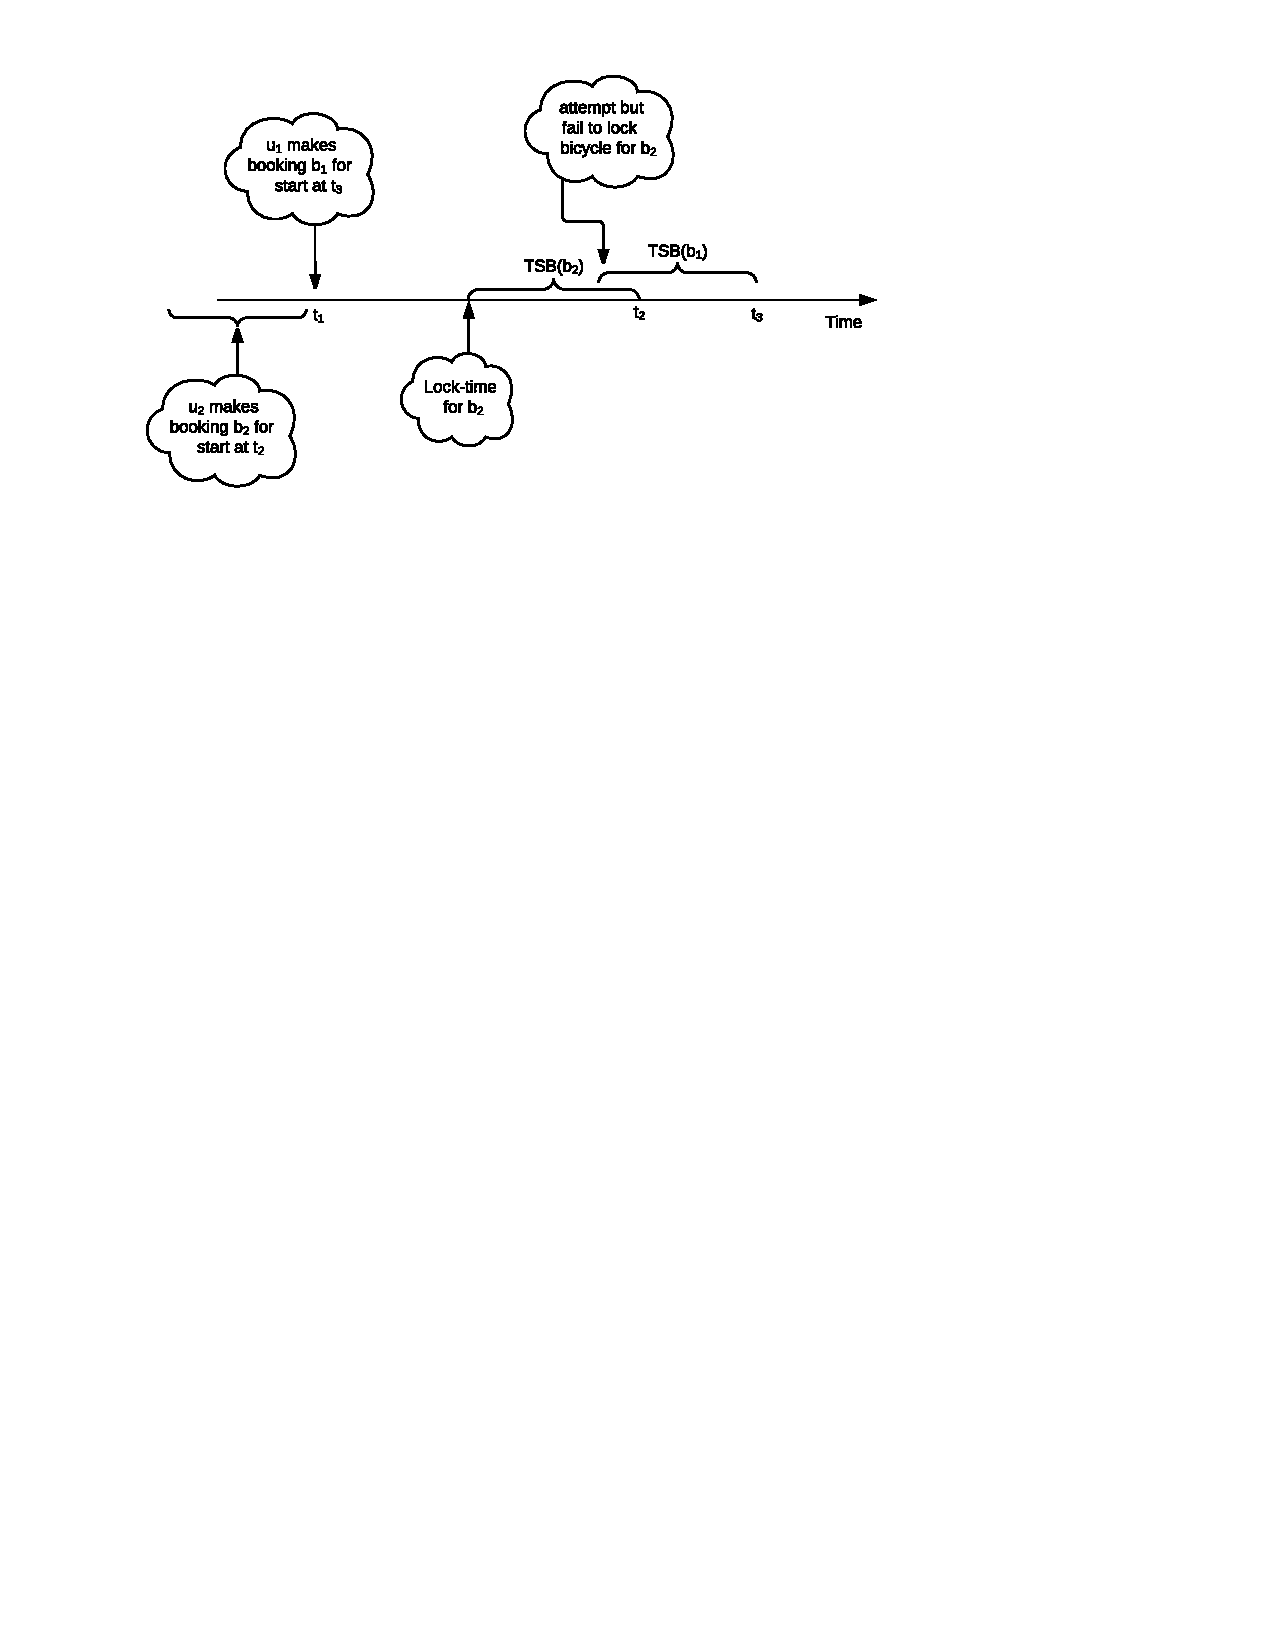
\includegraphics[trim = 1cm 19.7cm 0cm 0cm,clip]{behaviour/booking-illustration}
	\caption{Booking scenario illustration.}\label{fig:booking-illustartion}
\end{figure}
Then the scenario is given if $TSB(b_2)$ starts before $TSB(b_1)$ and $TSB(b_2)$ starts after $t_1$, we have a situation as can be seen in \figref{fig:booking-illustartion}.
As can be examined from the illustration, a problem occurs, under the assumption that no new bicycles gets delivered or taken from the given station in the given time-line, and where the amount of available bicycles before the lock-time of $b_2$ is 1.

The problem for user $u_1$ is then at time $t_1$ it appeared that a bicycle was available, but the bicycle is locked for user $u_2$ (although not entirely certain, see Problem 1.2) before it is locked for $u_1$ resulting in an availability count of 0 for $u_1$, thereby having no bicycle to lock for $u_1$.

\item[Problem 1.2] Having a booking system that is capable of capturing the state of each station, giving available bicycles and available free docks, along with the ability to borrow a bicycle without interacting with the booking system, imposes an element of unpredictability.

Given the scenario where a user reads the state of a station and makes a booking $b$ on that station at a time $t$ starting before $TSB(b)$, no certainty is provided that ensures that a bicycle is available to lock in $TSB(b)$. 
This is due to other users, who might have borrowed the rest of the bicycles at that station before $TSB(b)$, thus preventing the station from locking the desired amount of bicycles.

\fxwarning{Forstår det ikke, fungerer systemet sådan som det antager? Falder antal tilgængelig cykler ikke når man laver en booking?}
\item[Problem 1.3]
For how often a GPS have to read, some information have to be described before hand.
First it is necessary to decide what kind of information is desired from the GPS.
If the desired information is just current position of the bicycles, infrequent updates work just as well as frequent ones, however, if information about bicycle routes are what is desired, then more frequent updates would be necessary.

To illustrate this we can look at \figref{fig:gpsCircles}, the green circle in this picture is where the bicycle is at the last update, where the rings indicate where you can be after some seconds.
To look at time intervals the information of how often a GPS can reed have to be determined, this is determined by looking at datasheets of GPS, here a datasheet \citep{manual:gpsDataSheet} states that the GPS can read 50 times per second, therefore anything higher than that can be chosen.
In the figure the three circles represent 10 (blue), 30  (yellow), and 60 (red) seconds time intervals at a speed of 20 km/h.
The overlay on the map represents the distance that can be covered if travelling in a straight line, however, when travelling with a bicycle straight line travelling is not very common.
20 km/h was chosen as the speed because this is the average speed of bicycles where all the intersection lights are green \citep{misc:bicycleStatistics}.

We have chosen to let the GPS update at least every 30 second, since this makes it possible for us to determine the precise route of the bicycle.
The reason why 30 seconds was chosen is because you are not able to move that far in 10 seconds, however, when tracking only every 60 second it is possible to take alternative routes than the shortest route.


\begin{figure}
	\centering
	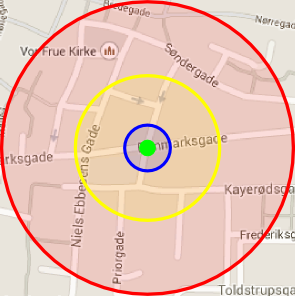
\includegraphics[scale=1]{GPScircles}
	\caption{Distance coverage with 20 km/h.}
	\label{fig:gpsCircles}
\end{figure}

\item[Problem 1.4]
As the stations and the website are located on different addresses and communication is through TCP, you have to consider how to synchronise the various parts of the system, in order to avoid an inconsistent state.

Several types of such inconsistent information could happen if you are not careful.

An scenario that could lead to an inconsistent state, if not handled well, is what happens when a station fails to communicate its current state to the global system.
A station maintains a local database holding information about each current booking made at that station.
When a booking has been processed, meaning that the user has taken the bicycle associated with the booking, the state of the local database changes in that the booking does not exist any more.
This change in state is also communicated to the global database maintained by the global system.
But when trying to communicate the change, the connection is interrupted due to a failure in the software at the station.

The problem is then, formulated with other words, which database holds the correct state of the overall system?
This depends highly on the direction of communication failure. 
In the described case above, the communication failure lies with the station software resulting in the local database of the station having the correct and current state of the system, which is when it comes to the state of the docks.


But if the direction of communication is the opposite, which would be involving bookings registered, the global system would have the correct booking information.

The desired behaviour of the system is to always be in a correct state, which requires that when a communication failure happens, the part participating in the communication holding the correct state resends its information, or the one with the inconsistent reads the state from the consistent counterpart.

There are two cases for the communication between the station software and the global system (web service).

\textbf{Station to Global System}\\
A communication failure in this direction results in a faulty state of how many bicycles are available at the given station thereby resulting in a rather useless website for booking.
Additionally, this can also involve the global system having the incorrect amount of docks registered, if such a change were performed at the station.

\textbf{Global System to Station}\\
A communication failure in this direction results in a failing booking system, in that no booking made at the website reaches the station and thereby have no effect at all.
In the end this gives a faulty state of how many bicycles are available at the given station because the station does not know of the booking and thereby not perform the necessary actions to make it a booking.

% station --> web : update, insert
% web --> station : insert, delete, update
\end{description}

